% Options for packages loaded elsewhere
\PassOptionsToPackage{unicode}{hyperref}
\PassOptionsToPackage{hyphens}{url}
%
\documentclass[
  english,
  man]{apa6}
\usepackage{lmodern}
\usepackage{amsmath}
\usepackage{ifxetex,ifluatex}
\ifnum 0\ifxetex 1\fi\ifluatex 1\fi=0 % if pdftex
  \usepackage[T1]{fontenc}
  \usepackage[utf8]{inputenc}
  \usepackage{textcomp} % provide euro and other symbols
  \usepackage{amssymb}
\else % if luatex or xetex
  \usepackage{unicode-math}
  \defaultfontfeatures{Scale=MatchLowercase}
  \defaultfontfeatures[\rmfamily]{Ligatures=TeX,Scale=1}
\fi
% Use upquote if available, for straight quotes in verbatim environments
\IfFileExists{upquote.sty}{\usepackage{upquote}}{}
\IfFileExists{microtype.sty}{% use microtype if available
  \usepackage[]{microtype}
  \UseMicrotypeSet[protrusion]{basicmath} % disable protrusion for tt fonts
}{}
\makeatletter
\@ifundefined{KOMAClassName}{% if non-KOMA class
  \IfFileExists{parskip.sty}{%
    \usepackage{parskip}
  }{% else
    \setlength{\parindent}{0pt}
    \setlength{\parskip}{6pt plus 2pt minus 1pt}}
}{% if KOMA class
  \KOMAoptions{parskip=half}}
\makeatother
\usepackage{xcolor}
\IfFileExists{xurl.sty}{\usepackage{xurl}}{} % add URL line breaks if available
\IfFileExists{bookmark.sty}{\usepackage{bookmark}}{\usepackage{hyperref}}
\hypersetup{
  pdftitle={Development of an Intentional BiFactor Engagement Measure},
  pdfauthor={Morgan Russell1, Casey Osorio-Duffoo2, Renata Garcia Prieto Palacios Roji1, \& John Kulas1},
  pdflang={en-EN},
  pdfkeywords={Engagement, engagement},
  hidelinks,
  pdfcreator={LaTeX via pandoc}}
\urlstyle{same} % disable monospaced font for URLs
\usepackage{graphicx}
\makeatletter
\def\maxwidth{\ifdim\Gin@nat@width>\linewidth\linewidth\else\Gin@nat@width\fi}
\def\maxheight{\ifdim\Gin@nat@height>\textheight\textheight\else\Gin@nat@height\fi}
\makeatother
% Scale images if necessary, so that they will not overflow the page
% margins by default, and it is still possible to overwrite the defaults
% using explicit options in \includegraphics[width, height, ...]{}
\setkeys{Gin}{width=\maxwidth,height=\maxheight,keepaspectratio}
% Set default figure placement to htbp
\makeatletter
\def\fps@figure{htbp}
\makeatother
\setlength{\emergencystretch}{3em} % prevent overfull lines
\providecommand{\tightlist}{%
  \setlength{\itemsep}{0pt}\setlength{\parskip}{0pt}}
\setcounter{secnumdepth}{-\maxdimen} % remove section numbering
% Make \paragraph and \subparagraph free-standing
\ifx\paragraph\undefined\else
  \let\oldparagraph\paragraph
  \renewcommand{\paragraph}[1]{\oldparagraph{#1}\mbox{}}
\fi
\ifx\subparagraph\undefined\else
  \let\oldsubparagraph\subparagraph
  \renewcommand{\subparagraph}[1]{\oldsubparagraph{#1}\mbox{}}
\fi
% Manuscript styling
\usepackage{upgreek}
\captionsetup{font=singlespacing,justification=justified}

% Table formatting
\usepackage{longtable}
\usepackage{lscape}
% \usepackage[counterclockwise]{rotating}   % Landscape page setup for large tables
\usepackage{multirow}		% Table styling
\usepackage{tabularx}		% Control Column width
\usepackage[flushleft]{threeparttable}	% Allows for three part tables with a specified notes section
\usepackage{threeparttablex}            % Lets threeparttable work with longtable

% Create new environments so endfloat can handle them
% \newenvironment{ltable}
%   {\begin{landscape}\centering\begin{threeparttable}}
%   {\end{threeparttable}\end{landscape}}
\newenvironment{lltable}{\begin{landscape}\centering\begin{ThreePartTable}}{\end{ThreePartTable}\end{landscape}}

% Enables adjusting longtable caption width to table width
% Solution found at http://golatex.de/longtable-mit-caption-so-breit-wie-die-tabelle-t15767.html
\makeatletter
\newcommand\LastLTentrywidth{1em}
\newlength\longtablewidth
\setlength{\longtablewidth}{1in}
\newcommand{\getlongtablewidth}{\begingroup \ifcsname LT@\roman{LT@tables}\endcsname \global\longtablewidth=0pt \renewcommand{\LT@entry}[2]{\global\advance\longtablewidth by ##2\relax\gdef\LastLTentrywidth{##2}}\@nameuse{LT@\roman{LT@tables}} \fi \endgroup}

% \setlength{\parindent}{0.5in}
% \setlength{\parskip}{0pt plus 0pt minus 0pt}

% \usepackage{etoolbox}
\makeatletter
\patchcmd{\HyOrg@maketitle}
  {\section{\normalfont\normalsize\abstractname}}
  {\section*{\normalfont\normalsize\abstractname}}
  {}{\typeout{Failed to patch abstract.}}
\patchcmd{\HyOrg@maketitle}
  {\section{\protect\normalfont{\@title}}}
  {\section*{\protect\normalfont{\@title}}}
  {}{\typeout{Failed to patch title.}}
\makeatother
\shorttitle{BiFactor Engagement}
\keywords{Engagement, engagement\newline\indent Word count: X}
\DeclareDelayedFloatFlavor{ThreePartTable}{table}
\DeclareDelayedFloatFlavor{lltable}{table}
\DeclareDelayedFloatFlavor*{longtable}{table}
\makeatletter
\renewcommand{\efloat@iwrite}[1]{\immediate\expandafter\protected@write\csname efloat@post#1\endcsname{}}
\makeatother
\usepackage{csquotes}
\ifxetex
  % Load polyglossia as late as possible: uses bidi with RTL langages (e.g. Hebrew, Arabic)
  \usepackage{polyglossia}
  \setmainlanguage[]{english}
\else
  \usepackage[shorthands=off,main=english]{babel}
\fi
\ifluatex
  \usepackage{selnolig}  % disable illegal ligatures
\fi
\newlength{\cslhangindent}
\setlength{\cslhangindent}{1.5em}
\newlength{\csllabelwidth}
\setlength{\csllabelwidth}{3em}
\newenvironment{CSLReferences}[2] % #1 hanging-ident, #2 entry spacing
 {% don't indent paragraphs
  \setlength{\parindent}{0pt}
  % turn on hanging indent if param 1 is 1
  \ifodd #1 \everypar{\setlength{\hangindent}{\cslhangindent}}\ignorespaces\fi
  % set entry spacing
  \ifnum #2 > 0
  \setlength{\parskip}{#2\baselineskip}
  \fi
 }%
 {}
\usepackage{calc}
\newcommand{\CSLBlock}[1]{#1\hfill\break}
\newcommand{\CSLLeftMargin}[1]{\parbox[t]{\csllabelwidth}{#1}}
\newcommand{\CSLRightInline}[1]{\parbox[t]{\linewidth - \csllabelwidth}{#1}\break}
\newcommand{\CSLIndent}[1]{\hspace{\cslhangindent}#1}

\title{Development of an Intentional BiFactor Engagement Measure}
\author{Morgan Russell\textsuperscript{1}, Casey Osorio-Duffoo\textsuperscript{2}, Renata Garcia Prieto Palacios Roji\textsuperscript{1}, \& John Kulas\textsuperscript{1}}
\date{}


\authornote{

Add complete departmental affiliations for each author here. Each new line herein must be indented, like this line.

Enter author note here.

Correspondence concerning this article should be addressed to Morgan Russell, Postal address. E-mail: \href{mailto:russellm5@montclair.edu}{\nolinkurl{russellm5@montclair.edu}}

}

\affiliation{\vspace{0.5cm}\textsuperscript{1} Montclair State University\\\textsuperscript{2} Harver}

\abstract{
Employee engagement has, in recent years, enjoyed a surge in popularity as a positive employee outcome.
Despite this burgeoning interest, disagreement still remains regarding its factor structure and nomological relationship with similar concepts, such as burnout.

One or two sentences providing a \textbf{basic introduction} to the field, comprehensible to a scientist in any discipline.

Two to three sentences of \textbf{more detailed background}, comprehensible to scientists in related disciplines.

One sentence clearly stating the \textbf{general problem} being addressed by this particular study.

One sentence summarizing the main result (with the words ``\textbf{here we show}'' or their equivalent).

Two or three sentences explaining what the \textbf{main result} reveals in direct comparison to what was thought to be the case previously, or how the main result adds to previous knowledge.

One or two sentences to put the results into a more \textbf{general context}.

Two or three sentences to provide a \textbf{broader perspective}, readily comprehensible to a scientist in any discipline.
}



\begin{document}
\maketitle

The roots of employee (aka work; e.g., W. Schaufeli \& Bakker, 2010) engagement research likely started with theoretical expansions of forms of employee participation (see, for example, Ferris \& Hellier, 1984) and job involvement (e.g., Elloy, Everett, \& Flynn, 1991). This exploration extended into broader considerations of attitudes and emotions (Staw, Sutton, \& Pelled, 1994) and were informed by further exploration of the dimensionality of constructs such as organizational commitment (Meyer \& Allen, 1991). The 1990's saw focused development and refinement (for example, a dissertation; Leone (1995) or actual semantic reference; Kahn (1990)). Staw, Sutton, and Pelled (1994) investigated the relationships between \emph{positive emotions} and favorable work outcomes, and although they do not use the word, ``engagement,'' their distinction between felt and expressed emotion likely held influence upon the burgeoning interest in the engagement construct.

Kahn (1990) described engaged employees as being physically involved, cognitively vigilant, and emotionally connected. Although occasionally referred to as residing on the opposing pole to \emph{burnout} (Christina Maslach \& Leiter, 2008), these two constructs are currently most commonly conceptualized as being distinct (Goering, Shimazu, Zhou, Wada, \& Sakai, 2017; Kim, Shin, \& Swanger, 2009; Wilmar B. Schaufeli, Taris, \& Van Rhenen, 2008; Timms, Brough, \& Graham, 2012), although certainly not universally (Cole, Walter, Bedeian, \& O'Boyle, 2012; Taris, Ybema, \& Beek, 2017). Comparing the two, Goering, Shimazu, Zhou, Wada, and Sakai (2017) concluded that they have a moderate (negative) association, but also distinct nomological networks. Wilmar B. Schaufeli, Taris, and Van Rhenen (2008) investigated both internal and external association indicators, concluding that engagement and burnout (as well as \emph{workaholism}) should be considered three distinct constructs.

Burnout can be defined as a psychological syndrome characterized by exhaustion (low energy), cynicism (low involvement), and inefficacy (low self-efficacy), which is experienced in response to chronic job stressors (e.g., Leiter \& Maslach, 2004; C. Maslach \& Leiter, 1997). Alternatively, engagement refers to an individual worker's involvement and satisfaction as well as enthusiasm for work (Harter, Schmidt, \& Hayes, 2002). W. B. Schaufeli and Bakker (2003) further specify a ``positive, fulfilling, work-related state of mind that is characterized by vigor, dedication, and absorption'' (p.~74). Via their conceptualization, vigor is described as high levels of energy and mental resilience while working. Dedication refers to being strongly involved in one's work and experiencing a sense of significance, enthusiasm, inspiration, pride, and challenge. Absorption is characterized by being fully concentrated and happily engrossed in one's work, whereby time passes quickly and one has difficulties with detaching oneself from work (Wilmar B. Schaufeli, Salanova, González-Romá, \& Bakker, 2002). The dimension of absorption has been noted as being influenced in conceptual specification by (Csikszentmihalyi, 1990)'s concept of ``flow.''

Regarding measurement, Gallup is widely acknowledged as an early pioneer in the measurement of the construct (see, for example, Coffman \& Harter, 1999). The Utrecht Work Engagement Scale (UWES) is another self-report questionnaire developed by W. B. Schaufeli and Bakker (2003) that directly assesses the vigor, dedication, and absorption elements.

\begin{quote}
we need to do some market research on the Q12: 1. what's the feedback report look like? (google images show one overall ``satsifaction'' score and/or one overall ``engagement'' score), 2. how much does it cost, 3. what are the 200 pulse items Gallup refers to? (6/7/21)
\end{quote}

Our conceptualization of work engagement is a mental state wherein employees\ldots{}

\begin{itemize}
\tightlist
\item
  \ldots feel energized (\textbf{Vigor})
\item
  \ldots are enthusiastic about the content of their work and the things they do (\textbf{Dedication})
\item
  \ldots are so immersed in their work activities that time seems compressed (\textbf{Absorption})
\end{itemize}

\hypertarget{methods}{%
\section{Methods}\label{methods}}

Choice of focus on BIC versus AIC discussed in Dziak, Coffman, Lanza, Li, and Jermiin (2020).

\hypertarget{participants}{%
\subsection{Participants}\label{participants}}

330 individuals provided ratings across 36 candidate items. These participants were gathered via snowball sampling, with an initial population of undergraduate and graduate students, as well as professional acquaintances of faculty members.

Participant job title, hours worked per week, and organizational tenure were recorded. Mean hours worked per week was \texttt{r\ mean(together\$\textasciigrave{}How\ many\ hours\ do\ you\ typically\ work\ per\ week\ in\ this\ job?\textasciigrave{},\ na.rm\ =\ TRUE)} . Mean organizational tenure was 6.82 years with a standard deviation of 8.50. Participants who did not exactly specify their tenure (e.g.~``A bit over a year'') were not included in this average.

\begin{figure}
\centering
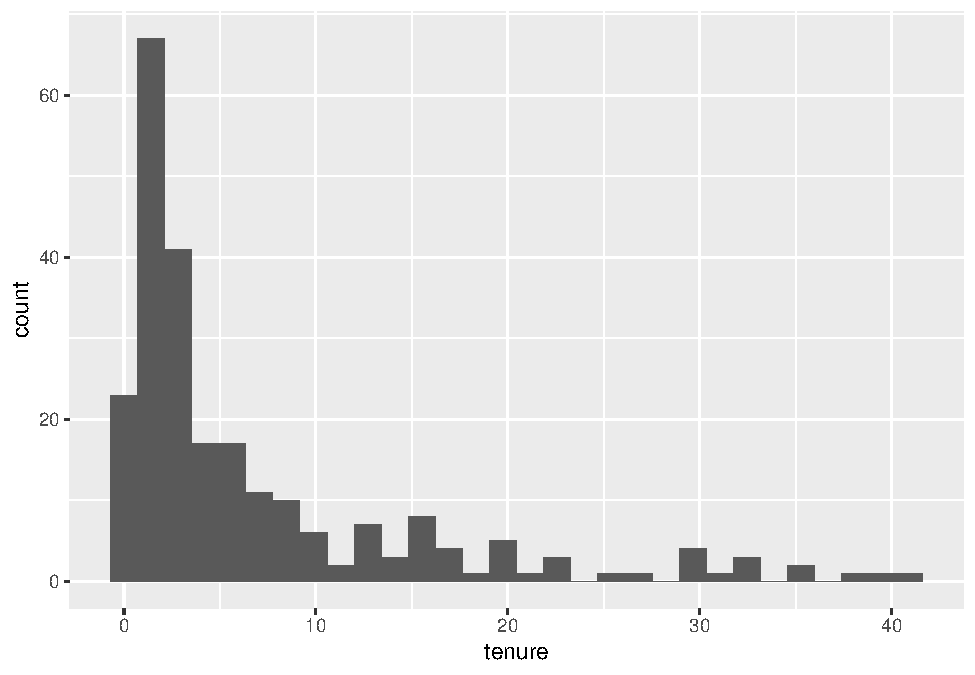
\includegraphics{SIOPpapaja_files/figure-latex/unnamed-chunk-1-1.pdf}
\caption{\label{fig:unnamed-chunk-1}Distribution of organizational tenure (years)}
\end{figure}

\begin{figure}
\centering
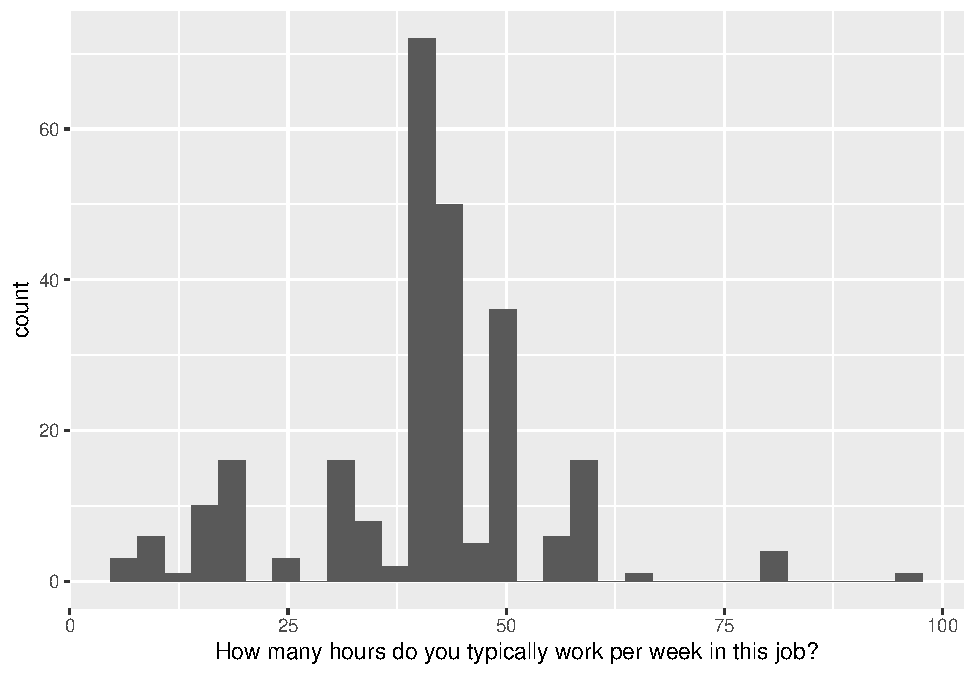
\includegraphics{SIOPpapaja_files/figure-latex/unnamed-chunk-2-1.pdf}
\caption{\label{fig:unnamed-chunk-2}Distribution of mean hours worked per week}
\end{figure}

Participants provided their job titles via an optional free text-entry box at the end of the survey. From there, we classified job titles according to the International Standard Classification of Occupations (ISCO-8) with the \texttt{classify\_occupation} function within the \texttt{labourR} package ((\textbf{kouretsis2020?})). The ISCO hierarchically organizes jobs in increasing order of specificity. For example, the first level of the hierarchy distinguishes a professional from a clerical worker or a technician. On the second level, professionals are distinguished among each other by whether they are engineers, medical workers, lawyers, and so on.

51, 120, 62, 4, 8, 1, and 3

\hypertarget{material}{%
\subsection{Material}\label{material}}

Our survey was administered on Qualtrics.

\hypertarget{item-generation}{%
\subsubsection{Item generation}\label{item-generation}}

We generated a set of 36 items for our engagement measure, with the ultimate goal of reducing them to a final set of 18. These items were generated according to a review of extant tripartite engagement measures, as well as \emph{WHAT RESEARCH DID WE USE FOR ATTITUDINAL WORDING? WAS IT LITERALLY JUST ``I THINK,'' ``I FEEL,'' ``I DO?''} Each item was worded to reflect both a substantive dimension as well as an attitudinal dimension, for example \emph{EXAMPLE ITEM HERE}

Our 3x3 bifactor model produced nine pairs of dimensions (e.g., Vigor-Cognitive, Vigor-Affective, Vigor-Behavioral, etc.). With 36 initial items, this left four items per pair of substantive and attitudinal dimensions.

The substantive scale definitions provided for ratings were:

\begin{itemize}
\item
  \emph{Absorption}: Being fully immersed in one's work, where time passes quickly and one has difficulty detaching from work tasks
\item
  \emph{Vigor}: Experiencing persistent levels of energy, effort, and enthusiasm while working
\item
  \emph{Dedication}: Experiencing pride and challenge in ones work, as well as strong feelings of support from and loyalty toward the organization
\end{itemize}

The attitudinal scale definitions were:

\begin{itemize}
\item
  \emph{Cognitive}: Pertaining to thoughts or general mental processes (for example what someone thinks)
\item
  \emph{Affective}: Pertaining to feelings or emotions (for example, how someone feels)
\item
  \emph{Behavioral}: Pertaining to acts or actions (for example, what someone does)
\end{itemize}

See table \emph{X} for a full list of items and their respective dimensions.

\hypertarget{procedure}{%
\subsection{Procedure}\label{procedure}}

\begin{quote}
Looking into the specification of polychoric covariances (Jöreskog, 1994). This seems to be not very commonly leveraged (only package that seems to estimate these is \texttt{semPlot}).
\end{quote}

The effective result of this was two divergent quasi-experimental approaches: 1) focus on corrected item-total correlations, and 2) focus on CFA modification indices.

\hypertarget{corrected-item-total-correlations}{%
\subsubsection{Corrected item-total correlations}\label{corrected-item-total-correlations}}

\begin{quote}
To Casey: document your process here
\end{quote}

\hypertarget{cfa-modification-indices}{%
\subsubsection{CFA Modification Indices}\label{cfa-modification-indices}}

We followed two parallel stepwise item-reduction processes centered around eliminating items in decreasing order of modification indices. Looking at the 36-item substantive and attitudinal models independently, we requested modification indices from each, with the intent of retaining indicators whose fixed shared residual covariances were associated with high modification indices (indicating better model fit if the paths were freed). The item pair with the highest modification index was scrutinized, with a subjective group judgment made on wording/semantics content domain coverage. The less preferred item was removed from the model. In cases where the highest modification index was between the only two remaining items in a substantive-attitudinal pair, these items were passed over for scrutiny in favor of the items with the next-highest index. This process was repeated until 18 items remained (i.e., 2 items for each of the 9 substantive-attitudinal pairs)

For example, the path with the highest modification index across both CFAs was between item 2 and item 4, which are both indicators of ``Absorption'' and ``Cognition.'' One of these items was therefore a candidate for deletion, and semantic preference was given to item 4, ``I find it difficult to mentally disconnect from work'' over item 2. After item 2 was excluded from both scale definitions (substantive and attitudinal), the CFAs were re-run and modification indices re-checked for bi-factor structure optimizing modifications.\footnote{Probably put a table in here highlighting certain modification indices (with a key to intended factor-item association). Look at ``modincides1''}

The end result was two separate final scale definitions (one optimized for the substantive model and one for the attitudinal).

We prioritized item deletions such that an item was implicated for deletion if: 1) modification index was high (relative to others) and 2) error residual was within same ``cell.'' The choice of item to delete was based on author preference for wording/semantics as well as construct element coverage (considering the possible consequences for construct deficiency). Item variance was also consulted (retention more likely with greater item variance).

\begin{table}[tbp]

\begin{center}
\begin{threeparttable}

\caption{\label{tab:unnamed-chunk-3}}

\begin{tabular}{llll}
\toprule
Variable 1 & \multicolumn{1}{c}{Relationship} & \multicolumn{1}{c}{Variable 2} & \multicolumn{1}{c}{<U+0394><U+03C7>2}\\
\midrule
Item\_2 & \textasciitilde{}\textasciitilde{} & Item\_4 & 192.41\\
Item\_8 & \textasciitilde{}\textasciitilde{} & Item\_18 & 96.05\\
Item\_29 & \textasciitilde{}\textasciitilde{} & Item\_35 & 62.25\\
Item\_14 & \textasciitilde{}\textasciitilde{} & Item\_20 & 56.38\\
Item\_1 & \textasciitilde{}\textasciitilde{} & Item\_12 & 51.39\\
Item\_1 & \textasciitilde{}\textasciitilde{} & Item\_13 & 50.33\\
\bottomrule
\end{tabular}

\end{threeparttable}
\end{center}

\end{table}

\begin{quote}
\begin{quote}
Actually it doesn't matter that much with only 1 item deletion - probably go ahead and do a few before recheck modification indices
\end{quote}
\end{quote}

\hypertarget{single-factor-versus-bifactor-approaches}{%
\subsubsection{Single factor versus bifactor approaches}\label{single-factor-versus-bifactor-approaches}}

\begin{quote}
Casey this is where you come in
\end{quote}

\hypertarget{data-analysis}{%
\subsection{Data analysis}\label{data-analysis}}

We used R {[}Version 4.1.0; R Core Team (2021){]} and the R-packages \emph{dplyr} {[}Version 1.0.6; Wickham, François, Henry, and Müller (2021){]}, \emph{DT} {[}Version 0.18; Xie, Cheng, and Tan (2021){]}, \emph{forcats} {[}Version 0.5.1; Wickham (2021a){]}, \emph{ggplot2} {[}Version 3.3.3; Wickham (2016){]}, \emph{kableExtra} {[}Version 1.3.4; Zhu (2021){]}, \emph{labourR} {[}Version 1.0.0; Kouretsis, Bampouris, Morfiris, and Papageorgiou (2020){]}, \emph{lavaan} {[}Version 0.6.8; Rosseel (2012){]}, \emph{magrittr} {[}Version 2.0.1; Bache and Wickham (2020){]}, \emph{papaja} {[}Version 0.1.0.9997; Aust and Barth (2020){]}, \emph{purrr} {[}Version 0.3.4; Henry and Wickham (2020){]}, \emph{readr} {[}Version 1.4.0; Wickham and Hester (2020){]}, \emph{sem} {[}Version 3.1.11; Fox, Nie, and Byrnes (2020); Epskamp (2019){]}, \emph{semPlot} {[}Version 1.1.2; Epskamp (2019){]}, \emph{stringr} {[}Version 1.4.0; Wickham (2019){]}, \emph{tibble} {[}Version 3.1.2; Müller and Wickham (2021){]}, \emph{tidyr} {[}Version 1.1.3; Wickham (2021b){]}, and \emph{tidyverse} {[}Version 1.3.1; Wickham et al. (2019){]} for all our analyses.

\hypertarget{results}{%
\section{Results}\label{results}}

CFA drafts below

\begin{figure}
\centering
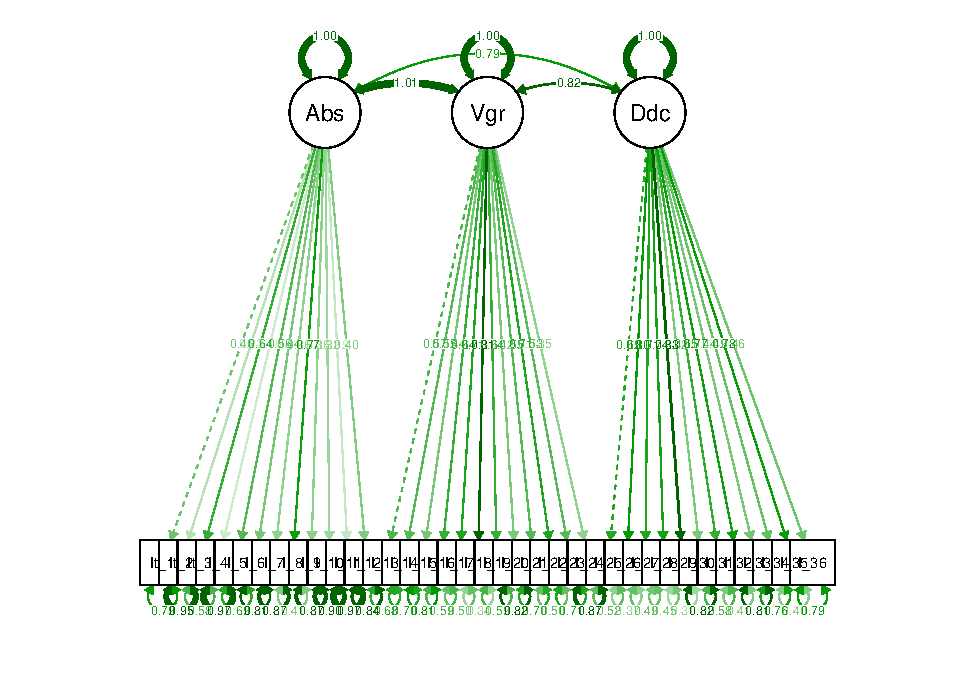
\includegraphics{SIOPpapaja_files/figure-latex/CFA.sub-1.pdf}
\caption{(\#fig:CFA.sub)Substantive factor structure CFA}
\end{figure}

\begin{figure}
\centering
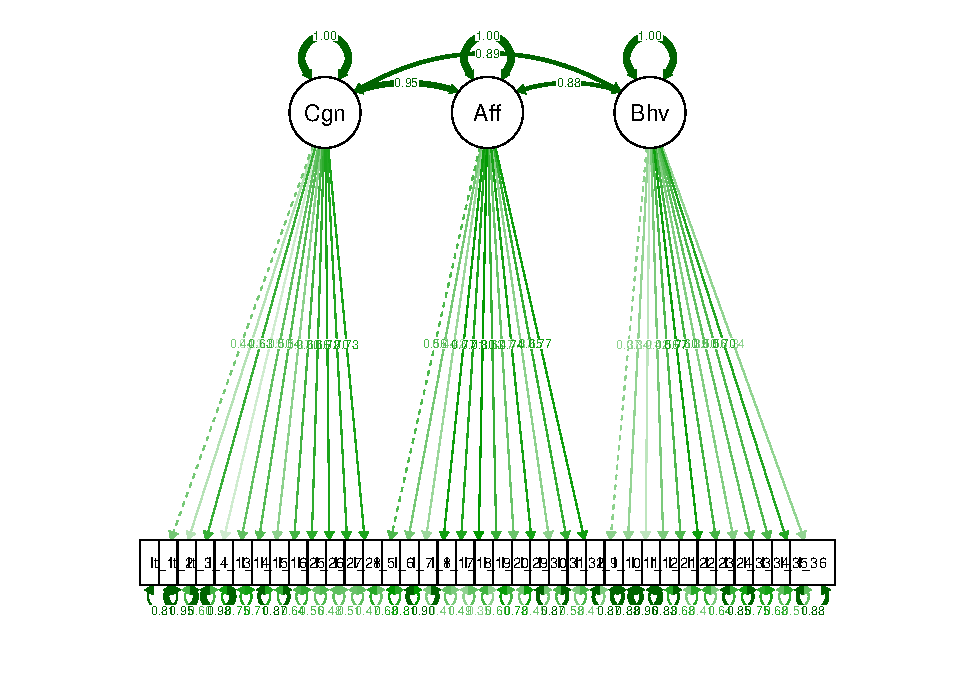
\includegraphics{SIOPpapaja_files/figure-latex/CFA.att-1.pdf}
\caption{(\#fig:CFA.att)Attitudinal factor structure CFA}
\end{figure}

\hypertarget{study-2}{%
\subsection{Study 2}\label{study-2}}

Construct validation was acccomplished via administration of the 17-item UWES as well as the Saks (2006) 12-item scale. Saks (2006) aggregates to two scales: job and organizational engagement.

\hypertarget{discussion}{%
\section{Discussion}\label{discussion}}

\newpage

\hypertarget{references}{%
\section{References}\label{references}}

\begingroup
\setlength{\parindent}{-0.5in}
\setlength{\leftskip}{0.5in}

\hypertarget{refs}{}
\begin{CSLReferences}{1}{0}
\leavevmode\hypertarget{ref-R-papaja}{}%
Aust, F., \& Barth, M. (2020). \emph{{papaja}: {Create} {APA} manuscripts with {R Markdown}}. Retrieved from \url{https://github.com/crsh/papaja}

\leavevmode\hypertarget{ref-R-magrittr}{}%
Bache, S. M., \& Wickham, H. (2020). \emph{Magrittr: A forward-pipe operator for r}. Retrieved from \url{https://CRAN.R-project.org/package=magrittr}

\leavevmode\hypertarget{ref-coffman_hard_1999}{}%
Coffman, C., \& Harter, J. (1999). A hard look at soft numbers. \emph{Position Paper, Gallup Organization}.

\leavevmode\hypertarget{ref-cole2012job}{}%
Cole, M. S., Walter, F., Bedeian, A. G., \& O'Boyle, E. H. (2012). Job burnout and employee engagement: A meta-analytic examination of construct proliferation. \emph{Journal of Management}, \emph{38}(5), 1550--1581.

\leavevmode\hypertarget{ref-csikszentmihalyi1990flow}{}%
Csikszentmihalyi, M. (1990). \emph{Flow: The psychology of optimal experience} (Vol. 1990). Harper \& Row New York.

\leavevmode\hypertarget{ref-dziak2020sensitivity}{}%
Dziak, J. J., Coffman, D. L., Lanza, S. T., Li, R., \& Jermiin, L. S. (2020). Sensitivity and specificity of information criteria. \emph{Briefings in Bioinformatics}, \emph{21}(2), 553--565.

\leavevmode\hypertarget{ref-elloy_examination_1991}{}%
Elloy, D. F., Everett, J. E., \& Flynn, W. R. (1991). An examination of the correlates of job involvement. \emph{Group \& Organization Studies}, \emph{16}(2), 160--177. \url{https://doi.org/10.1177/105960119101600204}

\leavevmode\hypertarget{ref-R-semPlot}{}%
Epskamp, S. (2019). \emph{semPlot: Path diagrams and visual analysis of various SEM packages' output}. Retrieved from \url{https://CRAN.R-project.org/package=semPlot}

\leavevmode\hypertarget{ref-ferris_added_1984}{}%
Ferris, R., \& Hellier, P. (1984). Added value productivity schemes and employee participation. \emph{Asia Pacific Journal of Human Resources}, \emph{22}(4), 35--44. \url{https://doi.org/10.1177/103841118402200406}

\leavevmode\hypertarget{ref-R-sem}{}%
Fox, J., Nie, Z., \& Byrnes, J. (2020). \emph{Sem: Structural equation models}. Retrieved from \url{https://CRAN.R-project.org/package=sem}

\leavevmode\hypertarget{ref-goering2017not}{}%
Goering, D. D., Shimazu, A., Zhou, F., Wada, T., \& Sakai, R. (2017). Not if, but how they differ: A meta-analytic test of the nomological networks of burnout and engagement. \emph{Burnout Research}, \emph{5}, 21--34.

\leavevmode\hypertarget{ref-harter_business-unit-level_2002}{}%
Harter, J. K., Schmidt, F. L., \& Hayes, T. L. (2002). Business-unit-level relationship between employee satisfaction, employee engagement, and business outcomes: A meta-analysis. \emph{Journal of Applied Psychology}, \emph{87}(2), 268.

\leavevmode\hypertarget{ref-harter_business-unit-level_2002}{}%
Harter, J. K., Schmidt, F. L., \& Hayes, T. L. (2002). Business-unit-level relationship between employee satisfaction, employee engagement, and business outcomes: A meta-analysis. \emph{Journal of Applied Psychology}, \emph{87}(2), 268.

\leavevmode\hypertarget{ref-R-purrr}{}%
Henry, L., \& Wickham, H. (2020). \emph{Purrr: Functional programming tools}. Retrieved from \url{https://CRAN.R-project.org/package=purrr}

\leavevmode\hypertarget{ref-joreskog1994estimation}{}%
Jöreskog, K. G. (1994). On the estimation of polychoric correlations and their asymptotic covariance matrix. \emph{Psychometrika}, \emph{59}(3), 381--389.

\leavevmode\hypertarget{ref-kahn_psychological_1990}{}%
Kahn, W. A. (1990). Psychological conditions of personal engagement and disengagement at work. \emph{Academy of Management Journal}, \emph{33}(4), 692--724.

\leavevmode\hypertarget{ref-kahn_psychological_1990}{}%
Kahn, W. A. (1990). Psychological conditions of personal engagement and disengagement at work. \emph{Academy of Management Journal}, \emph{33}(4), 692--724.

\leavevmode\hypertarget{ref-kim_burnout_2009}{}%
Kim, H. J., Shin, K. H., \& Swanger, N. (2009). Burnout and engagement: {A} comparative analysis using the {Big} {Five} personality dimensions. \emph{International Journal of Hospitality Management}, \emph{28}(1), 96--104. \url{https://doi.org/10.1016/j.ijhm.2008.06.001}

\leavevmode\hypertarget{ref-R-labourR}{}%
Kouretsis, A., Bampouris, A., Morfiris, P., \& Papageorgiou, K. (2020). \emph{labourR: Classify multilingual labour market free-text to standardized hierarchical occupations}. Retrieved from \url{https://CRAN.R-project.org/package=labourR}

\leavevmode\hypertarget{ref-leiter_areas_2004}{}%
Leiter, M., \& Maslach, C. (2004). Areas of worklife: A structured approach to organizational predictors of job burnout. In \emph{Research in occupational stress and well-being} (Vol. 3, pp. 91--134). \url{https://doi.org/10.1016/S1479-3555(03)03003-8}

\leavevmode\hypertarget{ref-leone_relation_1995}{}%
Leone, D. R. (1995). \emph{The relation of work climate, higher order need satisfaction, need salience, and causality orientations to work engagement, psychological adjustment, and job satisfaction} (PhD thesis). ProQuest Information \& Learning.

\leavevmode\hypertarget{ref-maslach1997causes}{}%
Maslach, C., \& Leiter, M. (1997). What causes burnout. \emph{Maslach C, Leiter MP. The Truth About Burnout: How Organizations Cause Personal Stress and What to Do about It. San Francisco, CA: Josey-Bass Publishers}, 38--60.

\leavevmode\hypertarget{ref-maslach_early_2008}{}%
Maslach, Christina, \& Leiter, M. P. (2008). Early predictors of job burnout and engagement. \emph{Journal of Applied Psychology}, \emph{93}(3), 498--512.

\leavevmode\hypertarget{ref-meyer_three-component_1991}{}%
Meyer, J. P., \& Allen, N. J. (1991). A three-component conceptualization of organizational commitment. \emph{Human Resource Management Review}, \emph{1}(1), 61--89.

\leavevmode\hypertarget{ref-R-tibble}{}%
Müller, K., \& Wickham, H. (2021). \emph{Tibble: Simple data frames}. Retrieved from \url{https://CRAN.R-project.org/package=tibble}

\leavevmode\hypertarget{ref-R-base}{}%
R Core Team. (2021). \emph{R: A language and environment for statistical computing}. Vienna, Austria: R Foundation for Statistical Computing. Retrieved from \url{https://www.R-project.org/}

\leavevmode\hypertarget{ref-R-lavaan}{}%
Rosseel, Y. (2012). {lavaan}: An {R} package for structural equation modeling. \emph{Journal of Statistical Software}, \emph{48}(2), 1--36. Retrieved from \url{https://www.jstatsoft.org/v48/i02/}

\leavevmode\hypertarget{ref-saks2006antecedents}{}%
Saks, A. M. (2006). Antecedents and consequences of employee engagement. \emph{Journal of Managerial Psychology}, \emph{21}(7), 600--619.

\leavevmode\hypertarget{ref-schaufeli_uwesutrecht_2003}{}%
Schaufeli, W. B., \& Bakker, A. B. (2003). {UWES}--utrecht work engagement scale: Test manual. \emph{Unpublished Manuscript: Department of Psychology, Utrecht University}, \emph{8}.

\leavevmode\hypertarget{ref-schaufeli_measurement_2002}{}%
Schaufeli, Wilmar B., Salanova, M., González-Romá, V., \& Bakker, A. B. (2002). The measurement of engagement and burnout: A two sample confirmatory factor analytic approach. \emph{Journal of Happiness Studies}, \emph{3}(1), 71--92.

\leavevmode\hypertarget{ref-schaufeli_measurement_2002}{}%
Schaufeli, Wilmar B., Salanova, M., González-Romá, V., \& Bakker, A. B. (2002). The measurement of engagement and burnout: A two sample confirmatory factor analytic approach. \emph{Journal of Happiness Studies}, \emph{3}(1), 71--92.

\leavevmode\hypertarget{ref-schaufeli2008workaholism}{}%
Schaufeli, Wilmar B., Taris, T. W., \& Van Rhenen, W. (2008). Workaholism, burnout, and work engagement: Three of a kind or three different kinds of employee well-being? \emph{Applied Psychology}, \emph{57}(2), 173--203.

\leavevmode\hypertarget{ref-schaufeli_conceptualization_2010}{}%
Schaufeli, W., \& Bakker, A. (2010). The conceptualization and measurement of work engagement. In W. Schaufeli, A. Bakker, \& M. Leiter (Eds.), \emph{Work engagement: A handbook of essential theory and research} (pp. 10--24). New York: Psychology Press.

\leavevmode\hypertarget{ref-staw_employee_1994}{}%
Staw, B. M., Sutton, R. I., \& Pelled, L. H. (1994). Employee positive emotion and favorable outcomes at the workplace. \emph{Organization Science}, \emph{5}(1), 51--71.

\leavevmode\hypertarget{ref-taris2017burnout}{}%
Taris, T. W., Ybema, J. F., \& Beek, I. van. (2017). Burnout and engagement: Identical twins or just close relatives? \emph{Burnout Research}, \emph{5}, 3--11.

\leavevmode\hypertarget{ref-timms2012burnt}{}%
Timms, C., Brough, P., \& Graham, D. (2012). Burnt-out but engaged: The co-existence of psychological burnout and engagement. \emph{Journal of Educational Administration}, \emph{50}(3), 327--345.

\leavevmode\hypertarget{ref-R-ggplot2}{}%
Wickham, H. (2016). \emph{ggplot2: Elegant graphics for data analysis}. Springer-Verlag New York. Retrieved from \url{https://ggplot2.tidyverse.org}

\leavevmode\hypertarget{ref-R-stringr}{}%
Wickham, H. (2019). \emph{Stringr: Simple, consistent wrappers for common string operations}. Retrieved from \url{https://CRAN.R-project.org/package=stringr}

\leavevmode\hypertarget{ref-R-forcats}{}%
Wickham, H. (2021a). \emph{Forcats: Tools for working with categorical variables (factors)}. Retrieved from \url{https://CRAN.R-project.org/package=forcats}

\leavevmode\hypertarget{ref-R-tidyr}{}%
Wickham, H. (2021b). \emph{Tidyr: Tidy messy data}. Retrieved from \url{https://CRAN.R-project.org/package=tidyr}

\leavevmode\hypertarget{ref-R-tidyverse}{}%
Wickham, H., Averick, M., Bryan, J., Chang, W., McGowan, L. D., François, R., \ldots{} Yutani, H. (2019). Welcome to the {tidyverse}. \emph{Journal of Open Source Software}, \emph{4}(43), 1686. \url{https://doi.org/10.21105/joss.01686}

\leavevmode\hypertarget{ref-R-dplyr}{}%
Wickham, H., François, R., Henry, L., \& Müller, K. (2021). \emph{Dplyr: A grammar of data manipulation}. Retrieved from \url{https://CRAN.R-project.org/package=dplyr}

\leavevmode\hypertarget{ref-R-readr}{}%
Wickham, H., \& Hester, J. (2020). \emph{Readr: Read rectangular text data}. Retrieved from \url{https://CRAN.R-project.org/package=readr}

\leavevmode\hypertarget{ref-R-DT}{}%
Xie, Y., Cheng, J., \& Tan, X. (2021). \emph{DT: A wrapper of the JavaScript library 'DataTables'}. Retrieved from \url{https://CRAN.R-project.org/package=DT}

\leavevmode\hypertarget{ref-R-kableExtra}{}%
Zhu, H. (2021). \emph{kableExtra: Construct complex table with 'kable' and pipe syntax}. Retrieved from \url{https://CRAN.R-project.org/package=kableExtra}

\end{CSLReferences}

\endgroup


\end{document}
